\documentclass[../Main.tex]{subfiles}

\begin{document}
\author{Diffraction} %use author for title of lesson
\date{Year 1 Topic 18} %use date to refer to topic in main booklet

%\section{Diffraction} %Section is the title of the lesson repeated, ready for the main contents page.

\begin{frame}{Double Slit Diffraction}
\begin{multicols}{2}
    Recall the set up for a double slit. What variables affected the interference pattern? 
    %\pause
    \begin{itemize}
        \item D - the distance from double slits to screen. Unit: meters
        \item a - the slit separation (from center to center). Unit: meters
        \item $\lambda$ - the wavelength of light. Unit: meters
    \end{itemize}
    How might the number of slits affect the outcome? %\pause
    --the interference pattern becomes less spread out, with more distinct maxima.
    \columnbreak
    \begin{figure}
        \centering
        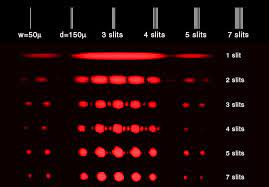
\includegraphics[height=4cm]{Waves_Images/7slitgrating.jpeg}
    \end{figure}
    Let's give it a go!
    \end{multicols}
\end{frame}

\begin{frame}{n-slit Diffraction}
The interference patterns for 1-5 slits would have an intensity profile as follows, where it is clear to see that there are more sharp peaks in intensity.
    \begin{figure}
        \centering
        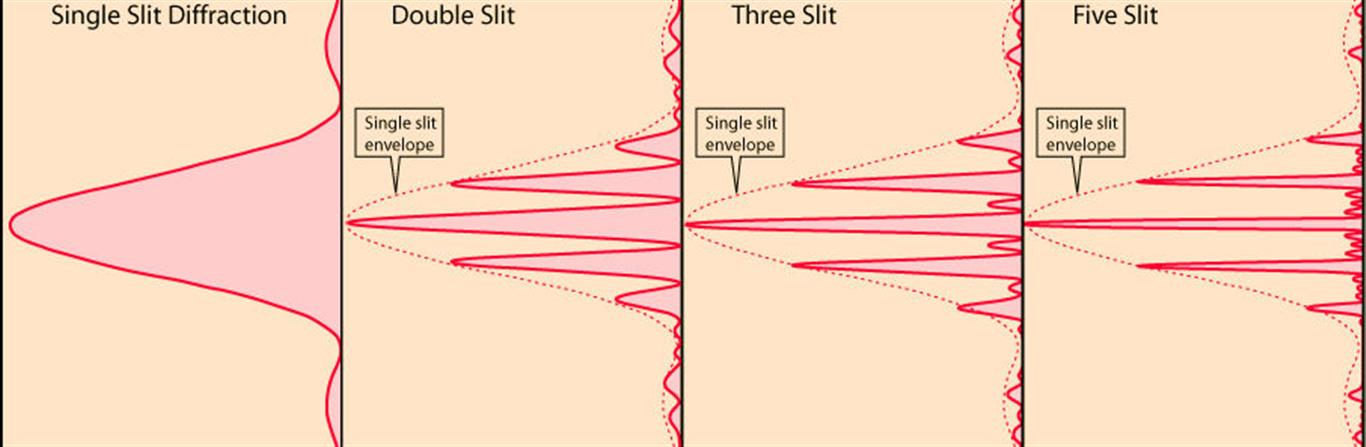
\includegraphics[width=\textwidth]{Waves_Images/5slitgraph.jpg}
    \end{figure}
    What might happen if we keep increasing the number of slits?
\end{frame}

\begin{frame}{Diffraction Grating}
    A diffraction grating creates an interference pattern, similar to a double slit, but with very distinct characteristics. As can be seen from the intensity profiles, as we increase the number of slits the maxima become more distinct, with more space between them. 
    %\pause
    \begin{figure}
        \centering
        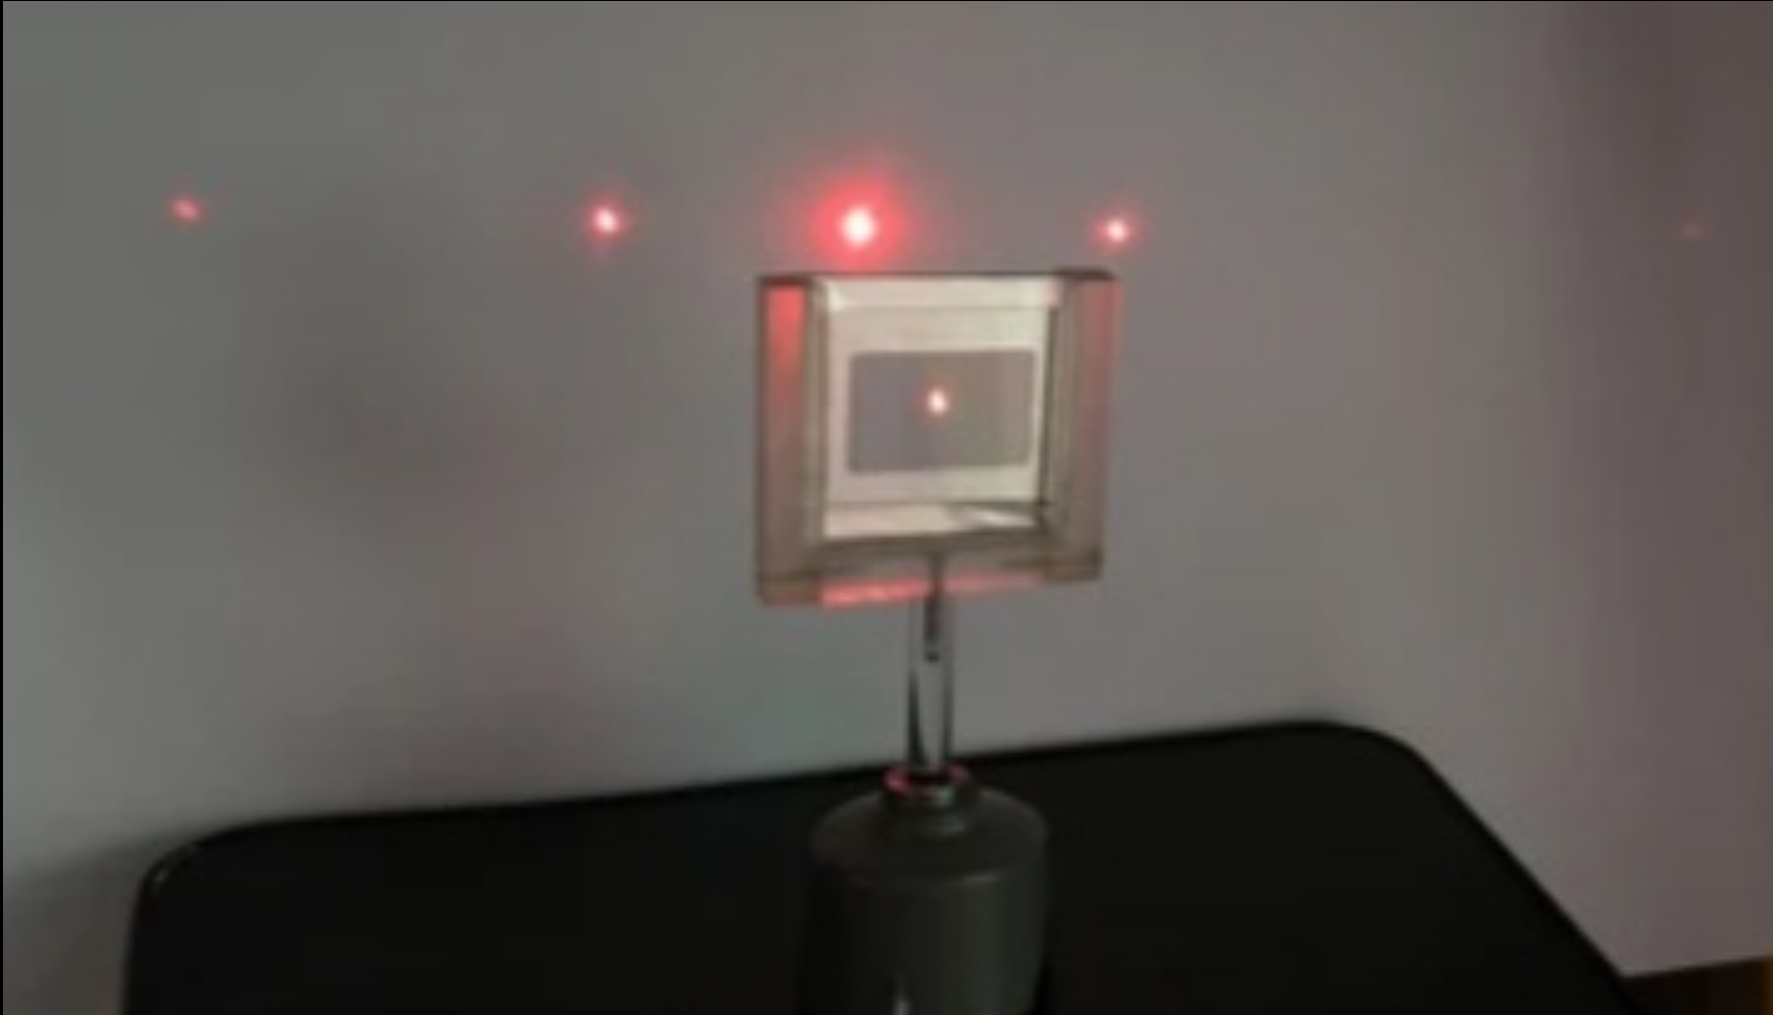
\includegraphics[width=0.6\textwidth]{Waves_Images/diffractiongrating.jpg}
    \end{figure}
    A diffraction grating simply creates a series of dots (or maxima).
\end{frame}

\begin{frame}{Diffraction Grating}
    A diffraction grating is a series of lines very close together - due to these lines we say that they are equivalent to having many slits -- of course then with some slit separation. 
    \begin{block}{Properties of a diffraction grating}
        A diffraction grating will have `x' lines per millimeter. In order to work out the line/slit separation, we must work out how many lines are present per meter, and take the inverse. 
    \end{block}
    \begin{exampleblock}{For example}
            600 lines per mm = $600\times 10^3$ lines per m, meaning the line separation is 1/$600\times 10^3 = 1.67\mu m$.
    \end{exampleblock}
\end{frame}

\begin{frame}{Diffraction Grating Formula}
    The diffraction grating formula is given as
    \begin{equation*}
        d sin\theta = n\lambda
    \end{equation*}
    where:
    \begin{itemize}
        \item d is the line separation in units meters
        \item $\theta$ is the angle of the order away from the central (n=0).
        \item n is the order in question, e.g. n=1,2,3...
        \item $\lambda$ is the wavelength of light.
    \end{itemize}
   %\pause
    \begin{exampleblock}{Example}
        Red light of wavelength 650nm is directed at a diffraction grating with 600 lines per mm. Calculate the angle from the central spot to all the orders visible. %\pause
        --$\theta = $ 29.9, 51.1
    \end{exampleblock}
\end{frame}

\begin{frame}{Monochromatic light}
    What do we think might happen if we compared different wavelengths of light? What might we expect to see different for a diffraction grating pattern for red vs blue light?
    %\pause
    \begin{figure}
        \centering
        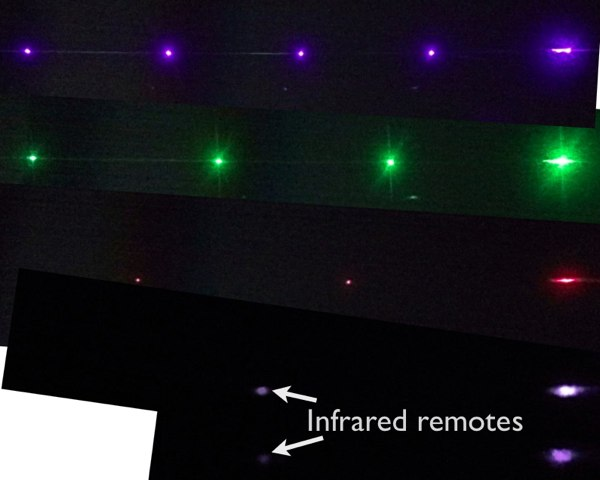
\includegraphics[width=5.5cm]{Waves_Images/differentlasersgrating.jpg}
    \end{figure}
    On the right-hand side here we see the central maxima n=0, and each subsequent order to the left. (This works for IR too, although we do not have IR lasers to play with!)
\end{frame}

\begin{frame}{White light}
    Up until now we have only considered and compared monochromatic light. What might happen if we shine white light through a diffraction grating? 
    %\pause
    \begin{figure}
        \centering
        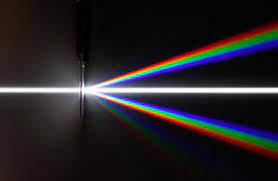
\includegraphics[width=8cm]{Waves_Images/whitelightgrating.jpeg}
    \end{figure}
    {\tiny (can anybody lend any pixels)}
\end{frame}

\begin{frame}{CDs}
    You might have seen this effect before but not realised it. The back of CDs/DVDs/Blu-rays are all mini diffraction gratings, only they reflect instead of transmit light.
    
    \begin{figure}
        \centering
        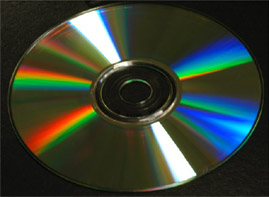
\includegraphics[width=8cm]{Waves_Images/cddiffract.jpg}
    \end{figure}
\end{frame}

\end{document}